\documentclass[conference]{IEEEtran}
\IEEEoverridecommandlockouts

\usepackage{cite}
\usepackage{amsmath,amssymb}
\usepackage{graphicx}
\usepackage{booktabs}
\usepackage{xcolor}
\usepackage{url}

% Values still being computed are marked in red; search for \pending before submission.
\newcommand{\pending}[1]{\textcolor{red}{[#1]}}
\graphicspath{{figures/}}

\begin{document}

\title{When Fine-Tuning Hurts in the Field: Adaptive Gating Between Frozen and Fine-Tuned Features for Plant Disease Recognition}

\author{\IEEEauthorblockN{Amrita Jena}
\IEEEauthorblockA{\textit{Department} \\
\textit{Institution}\\
City, Country \\
email}}

\maketitle

\begin{abstract}
Plant disease classifiers routinely exceed 99\% accuracy on the PlantVillage benchmark yet fail on photographs taken in the field. We study this gap under a leakage-controlled protocol: near-duplicate images are grouped by 64-bit perceptual hashes over all 1.47 billion image pairs, splits and cross-validation folds respect those groups, and field accuracy is measured on PlantDoc, which no model sees during training. Three current backbones---ConvNeXt-V2, MobileNetV4 and Swin-V2---are tuned with Optuna and evaluated with grouped cross-validation. Every fine-tuned model reaches 99.77--99.88\% on held-out PlantVillage images but only 21.6--32.3\% on PlantDoc. A linear probe on frozen ConvNeXt-V2 features loses two points in the laboratory (97.75\%) yet reaches 47.69\% in the field, 15.4 points above the best fine-tuned model, reproducing the feature-distortion effect of Kumar et al.\ in agriculture at large magnitude. We propose Adaptive Gated Fine-Tuning (AGFT), which keeps a frozen and a fine-tuned branch and learns a per-image gate from the frozen features, and evaluate it against plain fine-tuning, a linear probe and a learned fixed trade-off within one architecture. A fixed trade-off learns a weight of 0.507 and behaves like plain fine-tuning in the field (29.83\%). The learned gate reaches \pending{X}\% on PlantVillage and \pending{Y}\% on PlantDoc; an inference-only analysis shows how it weighs the two branches on laboratory and field images.
\end{abstract}

\begin{IEEEkeywords}
plant disease recognition, domain shift, fine-tuning, linear probing, gating, data leakage
\end{IEEEkeywords}

\section{Introduction}
Image-based plant disease recognition has reported near-perfect accuracy since convolutional networks were first applied to PlantVillage~\cite{hughes2015plantvillage,mohanty2016using}. The same studies observed the catch: models trained on laboratory images, photographed leaf by leaf on uniform backgrounds, transfer poorly to images taken in the field~\cite{mohanty2016using,ferentinos2018deep}. PlantDoc~\cite{singh2020plantdoc} was collected to measure exactly this. Laboratory accuracy has therefore stopped being informative: every modern architecture saturates it, and differences between models fall within the noise.

A separate line of work explains why fine-tuning in particular may be the problem. Kumar et al.~\cite{kumar2022finetuning} showed that fine-tuning distorts pretrained features and can underperform a linear probe out of distribution; their LP-FT remedy, and WiSE-FT's interpolation of fine-tuned and pretrained weights~\cite{wortsman2022robust}, choose \emph{one} trade-off between the pretrained and the fine-tuned solution for every input. Which branch is better, however, depends on the image: a laboratory-like photograph favours the fine-tuned features, an unfamiliar field photograph may favour the pretrained ones.

This paper makes four contributions.
\begin{itemize}
\item A leakage-controlled evaluation protocol for plant disease recognition: near-duplicate grouping with an explicit threshold-sensitivity analysis, grouped splits and grouped cross-validation, verified pair by pair, and both open-set and closed-set field evaluation.
\item A controlled comparison of three current backbones showing that laboratory accuracy saturates while field accuracy separates them, and that a frozen linear probe outperforms every fine-tuned model in the field by more than 15 points.
\item Adaptive Gated Fine-Tuning (AGFT), which routes each image between a frozen and a fine-tuned branch, together with the ablations that make the claim falsifiable: the gate pinned to one (fine-tuning), to zero (linear probe), and to a learned constant (a fixed trade-off).
\item An inference-only analysis of the learned gate: each branch alone, every fixed trade-off including a hindsight oracle, and where the gate sends laboratory and field images.
\end{itemize}

\section{Related Work}
\textbf{Plant disease recognition.} PlantVillage~\cite{hughes2015plantvillage} enabled the first deep models for the task~\cite{mohanty2016using}, and subsequent work reported accuracies above 99\%~\cite{ferentinos2018deep}. Both studies noted a large drop on field images; PlantDoc~\cite{singh2020plantdoc} provides 2,598 web-sourced field images across 27 classes for evaluating it.

\textbf{Robust fine-tuning.} Linear probes and full fine-tuning trade in-distribution accuracy against robustness~\cite{kornblith2019better,kumar2022finetuning}. LP-FT~\cite{kumar2022finetuning} fine-tunes after first fitting a linear head; WiSE-FT~\cite{wortsman2022robust} interpolates fine-tuned and pretrained weights with one global coefficient; side-tuning~\cite{zhang2020sidetuning} adds a trainable side network to a frozen base. All apply the same combination to every input.

\textbf{Gating.} Input-dependent mixtures of predictors date back to adaptive mixtures of local experts~\cite{jacobs1991adaptive} and scale to sparsely gated mixtures~\cite{shazeer2017outrageously}. AGFT applies this idea to a different pair of experts: one model's pretrained features, kept frozen, and the same model fine-tuned.

\section{Method}
\subsection{Adaptive Gated Fine-Tuning}
Let $B_f$ be a pretrained backbone kept frozen and $B_t$ a copy fine-tuned on the task, with linear heads $H_f$ and $H_t$. For an image $x$, AGFT computes
\begin{equation}
g(x) = \sigma\big(\mathrm{MLP}(B_f(x))\big), \quad
z(x) = g(x)\, H_t(B_t(x)) + \big(1 - g(x)\big)\, H_f(B_f(x)),
\label{eq:agft}
\end{equation}
where $\sigma$ is the logistic function and $z$ are the class logits. The gate is a two-layer MLP (768 to 96 units, GELU, to one output). It reads the \emph{frozen} features deliberately: they are the only description of the input whose statistics do not move while $B_t$ is being trained, so the gate sees a stable signal of how familiar an image is.

\subsection{Ablations Within One Architecture}
The same class implements four settings of $g$: $g{=}1$ is plain fine-tuning; $g{=}0$ is a linear probe on frozen features; $g{=}\sigma(a)$ with one learned scalar $a$ is a fixed trade-off in logit space, the output-space analogue of WiSE-FT; and the learned $g(x)$ of~\eqref{eq:agft} is AGFT. If AGFT cannot outperform the fixed trade-off, the per-image gate adds nothing.

\section{Experimental Protocol}
\subsection{Datasets}
PlantVillage is used in a public release of 55,447 images over 39 classes; the \textit{Background\_without\_leaves} class is removed because it contains no plant, leaving 54,304 images over 38 classes (imbalance ratio 36.2). PlantDoc annotates individual leaves; an image's label is the category its annotations agree on. The 20 images whose annotations disagree are excluded, leaving 2,558 images. A bridge maps its 29 categories onto PlantVillage class names; 27 of the 38 classes occur. Both datasets are pinned to fixed revisions.

\subsection{Leakage Control}
PlantVillage contains repeated photographs of the same leaf. Each image receives a 64-bit difference hash~\cite{zauner2010phash}, and all 1,474,435,056 pairs are compared exactly. Two images whose hashes differ in at most four bits are near-duplicates, and connected chains of such pairs form groups. Table~\ref{tab:dup} shows the threshold sensitivity: exact matching links only 46 images, four bits link 883 in 401 groups of at most 11, and at six bits chaining merges 820 images into one group, which would distort stratification. Whole groups are assigned to a stratified 70/15/15 split (37,990/8,145/8,169 images), and the split is verified pair by pair: no two images in different splits lie within four bits.

\begin{table}[t]
\caption{Near-duplicate grouping as a function of the hash threshold}
\label{tab:dup}
\centering
\begin{tabular}{@{}cccc@{}}
\toprule
Bits allowed to differ & Images in groups & Groups & Largest group \\
\midrule
0 & 46 & 23 & 2 \\
2 & 134 & 66 & 4 \\
3 & 360 & 175 & 5 \\
\textbf{4 (used)} & \textbf{883} & \textbf{401} & \textbf{11} \\
5 & 2,181 & 856 & 34 \\
6 & 5,149 & 1,530 & 820 \\
\bottomrule
\end{tabular}
\end{table}

\begin{figure*}[t]
\centering
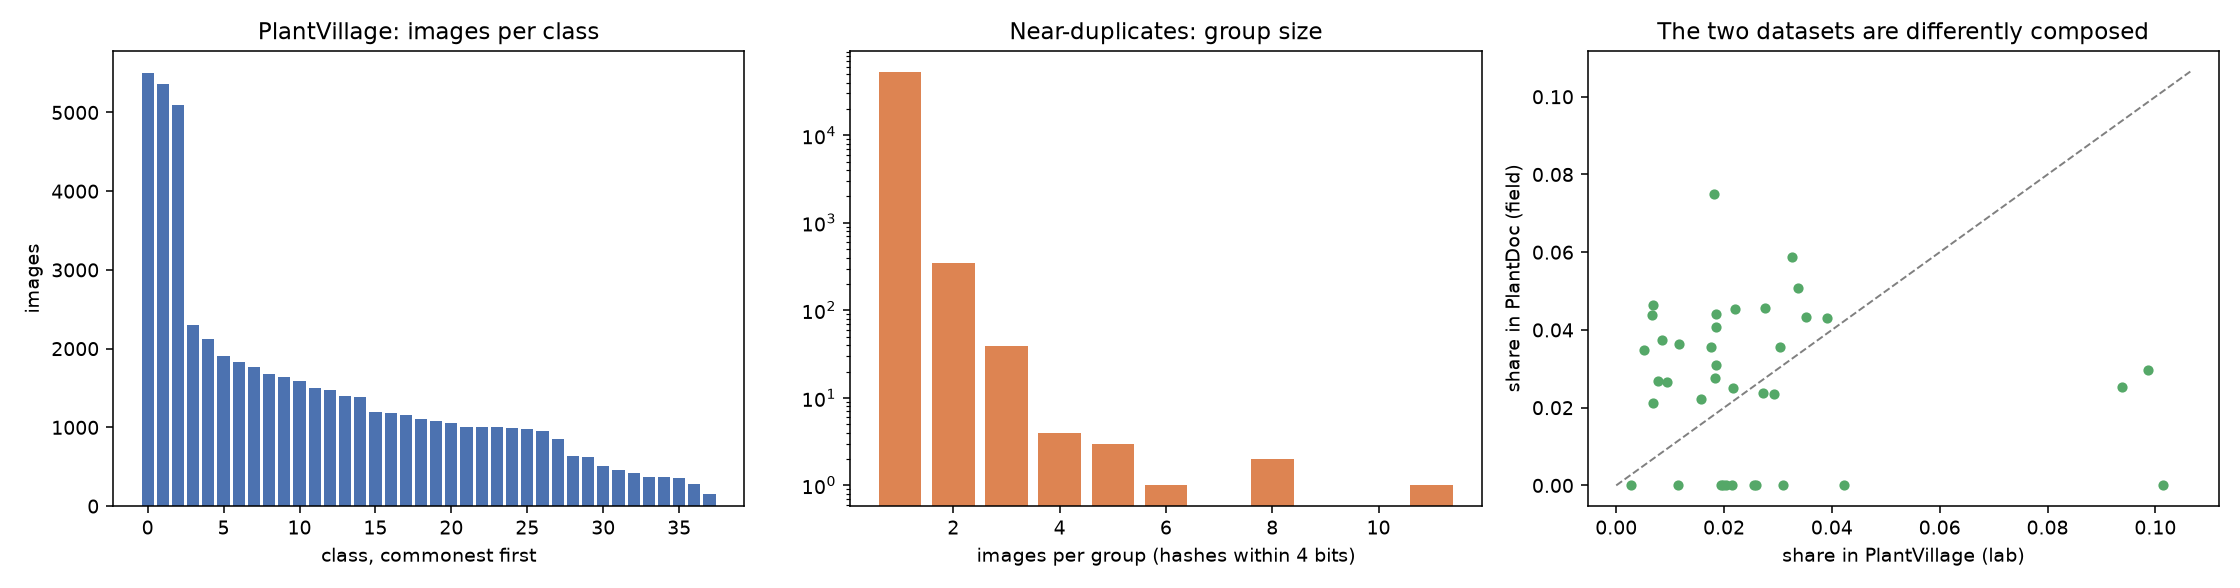
\includegraphics[width=\textwidth]{eda.png}
\caption{The data. Left: PlantVillage images per class (imbalance ratio 36.2). Centre: near-duplicate group sizes at the four-bit threshold (log scale). Right: class shares in PlantVillage against PlantDoc; the datasets are composed very differently.}
\label{fig:eda}
\end{figure*}

\subsection{Models and Training}
The backbones are ConvNeXt-V2-T~\cite{woo2023convnextv2} (27.9M parameters), MobileNetV4-Conv-M~\cite{qin2024mobilenetv4} (8.4M) and Swin-V2-T~\cite{liu2022swinv2} (27.6M), from timm~\cite{wightman2019timm}. Swin-V2 is rebuilt for 224-pixel input with a $7{\times}7$ window, which its continuous position bias supports. AGFT uses ConvNeXt-V2-T for both branches. All models train with AdamW, a one-epoch warm-up and cosine decay, bfloat16 mixed precision, batch size 64 and standard augmentation; early stopping monitors validation macro-F1 with patience three. Learning rate, weight decay and dropout are tuned per arm with Optuna~\cite{akiba2019optuna} (ten trials of three epochs on a 20\% training subset, median pruning). Each arm is then evaluated by grouped five-fold cross-validation on the training split (eight epochs per fold), trained once on the full training split, and tested once. All experiments ran on a single NVIDIA L4 GPU.

Because of a compute deadline, the learned-gate arm deviates in two documented ways: its cross-validation was stopped after three of the five folds, and its final fit used eight epochs (the budget of its folds) instead of twelve. The six other arms follow the full protocol.

\subsection{Evaluation}
In-distribution performance is accuracy and macro-F1 on the PlantVillage test split. Field performance is accuracy on all PlantDoc images, both \emph{open-set} (all 38 outputs, as a deployed model would face) and \emph{closed-set} (outputs restricted to the 27 classes PlantDoc contains, as most prior work reports).

\section{Results}
\begin{table*}[t]
\caption{Main results (\%). CV is grouped cross-validation macro-F1 on the training split (mean $\pm$ s.d.). Gate is the mean $g(x)$ on PlantDoc.}
\label{tab:main}
\centering
\begin{tabular}{@{}lccccc@{}}
\toprule
& CV macro-F1 & PlantVillage test & PlantDoc open-set & PlantDoc closed-set & Gate \\
\midrule
ConvNeXt-V2-T & 99.73 $\pm$ 0.06 & 99.77 & 32.25 & 36.00 & -- \\
MobileNetV4-M & 99.60 $\pm$ 0.07 & 99.83 & 21.62 & 25.53 & -- \\
Swin-V2-T & 99.66 $\pm$ 0.09 & 99.80 & 25.45 & 32.45 & -- \\
\midrule
AGFT, $g{=}1$ (fine-tune) & 99.74 $\pm$ 0.08 & 99.88 & 29.24 & 34.79 & -- \\
AGFT, $g{=}0$ (linear probe) & 96.67 $\pm$ 0.11 & 97.75 & \textbf{47.69} & \textbf{50.74} & -- \\
AGFT, fixed $\alpha$ & 99.69 $\pm$ 0.05 & 99.82 & 29.83 & 34.52 & 0.507 \\
AGFT, learned gate (ours) & 99.70 $\pm$ 0.07$^{\dagger}$ & \pending{X} & \pending{Y} & \pending{Z} & \pending{g} \\
\bottomrule
\multicolumn{6}{@{}l@{}}{\footnotesize $^{\dagger}$Three of five folds; final fit eight epochs instead of twelve (see Section IV-C).}
\end{tabular}
\end{table*}

\begin{figure*}[t]
\centering
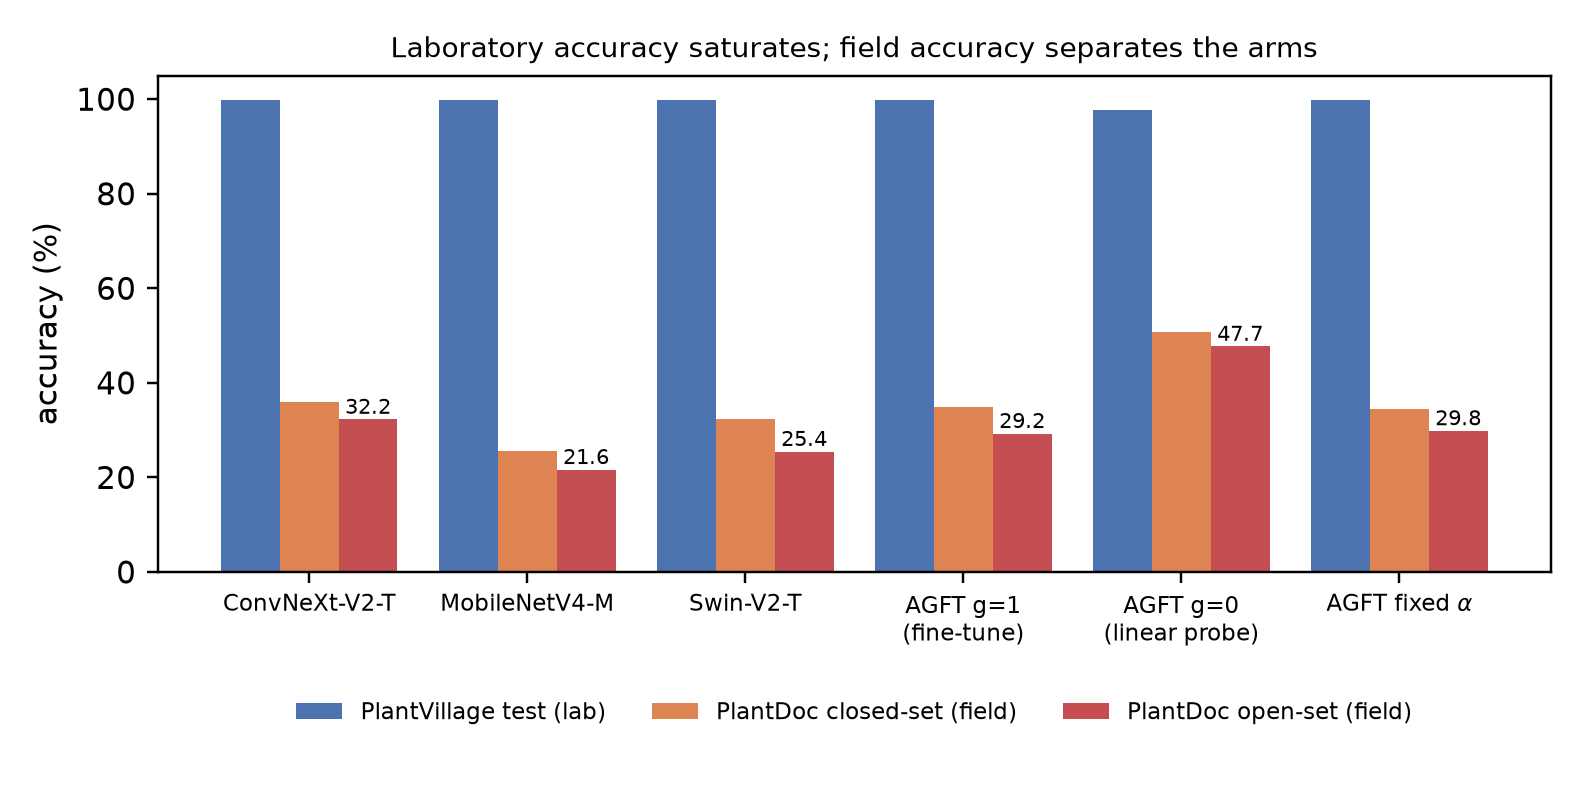
\includegraphics[width=0.85\textwidth]{lab_vs_field.png}
\caption{Laboratory against field accuracy for the six arms that completed the full protocol. Every arm scores 97.75--99.88\% on PlantVillage; on PlantDoc they span 21.62--47.69\%, and the frozen linear probe leads.}
\label{fig:labfield}
\end{figure*}

Table~\ref{tab:main} and Fig.~\ref{fig:labfield} report the arms. Three findings stand out.

\textbf{Laboratory accuracy cannot rank models.} Every fine-tuned arm lands between 99.77\% and 99.88\% on the PlantVillage test split, and cross-validation spreads are 0.05--0.09 points. On PlantDoc the same models span 21.62\% to 32.25\%, and their order changes: MobileNetV4, the best in the laboratory, is the worst in the field.

\textbf{Frozen features generalise far better.} The linear probe on frozen ConvNeXt-V2 features is the weakest arm in the laboratory (97.75\%) and the strongest in the field: 47.69\% open-set and 50.74\% closed-set, 15.44 and 14.74 points above the best fine-tuned model and 18.45 points above fine-tuning the same backbone inside the same architecture. Fine-tuning buys two laboratory points at the cost of fifteen field points, a far larger instance of the effect described by Kumar et al.~\cite{kumar2022finetuning}.

\textbf{A fixed trade-off behaves like fine-tuning.} The learned constant settles at $\sigma(a){=}0.507$, nearly equal weight on both branches, yet its field accuracy (29.83\%) is within a point of plain fine-tuning (29.24\%) and 18 points below the probe. A mixture in logit space is weighted by the branches' logit magnitudes as well as by the gate, so a confident fine-tuned branch dominates an even split.

\textbf{The learned gate.} \pending{Result of the learned gate on PlantVillage and PlantDoc, compared with the fixed trade-off and the linear probe.}

\subsection{What the Gate Does}
Table~\ref{tab:gate} and Fig.~\ref{fig:gate} decompose the trained AGFT model by inference alone. \pending{Interpretation: each branch alone; the learned gate against every fixed alpha including the oracle; the gate on laboratory versus field images (Mann--Whitney test~\cite{mann1947test}); the gate where only one branch is right; logit scales.}

\begin{table}[t]
\caption{Decomposition of the trained AGFT model (accuracy, \%)}
\label{tab:gate}
\centering
\begin{tabular}{@{}lcc@{}}
\toprule
& PlantVillage test & PlantDoc \\
\midrule
\pending{rows from results/table\_gate.tex} & & \\
\bottomrule
\end{tabular}
\end{table}

\begin{figure*}[t]
\centering
\IfFileExists{figures/gate_analysis.png}{\includegraphics[width=\textwidth]{gate_analysis.png}}{\pending{figure produced by notebook cell 13 as figures/gate\_analysis.png}}
\caption{The learned gate. Left: distribution of $g(x)$ on PlantVillage test and PlantDoc images. Centre: PlantDoc accuracy for every fixed trade-off $\alpha$, in logit and probability space, with the learned gate marked. Right: mean gate on PlantDoc images grouped by which branch classifies them correctly.}
\label{fig:gate}
\end{figure*}

\section{Discussion and Limitations}
The central practical finding is that, for plant disease recognition under domain shift, how a pretrained model is adapted matters more than which current architecture is chosen: the spread between adaptation strategies on one backbone (18.45 points) exceeds the spread between architectures (10.63 points). Laboratory benchmarks hide both.

The study has limitations. It uses one laboratory dataset and one field dataset; PlantDoc images are web-sourced, and its label bridge requires judgement for some categories. Each arm was trained with one seed. AGFT is evaluated on one backbone, and the learned-gate arm used a shortened protocol (Section IV-C). AGFT also doubles inference cost, since both branches run on every image.

\section{Conclusion}
Under a leakage-controlled protocol, three current backbones are indistinguishable on PlantVillage and far apart on PlantDoc, and a frozen linear probe outperforms all of them in the field by more than fifteen points. A fixed trade-off between frozen and fine-tuned features collapses to fine-tuning. \pending{Conclusion on the learned gate.} Field evaluation, not laboratory accuracy, should decide how plant disease models are built and adapted.

\bibliographystyle{IEEEtran}
\bibliography{refs}

\end{document}
